\subsection{Thermodynamische Potentiale}
\subsubsection{Legendre-Transformation}

\begin{itemize}[align=left]
  \item[\uline{Erinnerung}:] klassische Mechanik mit Lagrange-Funktion $L\norBra{q,\dot{q},t}$ und Impuls $p = \ppv{L}{\dot{q}}$\\
  $\rightarrow$ Hamiltonfunktion $H\norBra{q,p,t} = p\dot{q}\norBra{q,p} - L \norBra{q,\dot{q}\norBra{q,p},t}$
  \item[\uline{Schnelle Herleitung in der Thermodynamik}:] \begin{itemize}[align=left]
    \item[Umformung]$\dd{E} = T\dd{S} -p \dd{V} + \mu\dd{N} = \dd{ST} - S\dd{T} - p\dd{V} + \mu\dd{N}$
    \item[Erkenntnis]$\dd{\norBra{E-ST}} = - S\dd{T} -p \dd{V} + \mu\dd{N}$
    \item[Definition]$\rightarrow$ Definiere neue Funktion $F\mDef E-ST$ mit Variablen $T$, $V$, $N$.
    \item[Motivation:] Variable $T$ ist praktischer als $S$ (Messbarkeit, Anschaulichkeit)
  \end{itemize}
  \item[\uline{Mathematisch}:] \begin{itemize}[align=left]
    \item[Funktion] $f: x \mapsto f\norBra{x}$, $x\in\mathds{R}$, $f\norBra{x} \in\mathds{R}$
    \item[Annahme:] $\xi = f'\norBra{x} \mDef \ddv{f}{x}\norBra{x}$ existiert und $f''\norBra{x} \neq 0$ $\forall x$ $\rightarrow$ $x = \varphi\norBra{\xi}$
    \item[Definiere:] $h\norBra{\xi} \mDef f\norBra{\varphi\norBra{\xi}}$
    \item[Problem:] $h$ enthält \glqq weniger Informationen\grqq\ als $f$.
    \item[Gemeint:] $f$ kann nicht mehr eindeutig aus $h$ zurückgewonnen werden.
  \end{itemize}
\end{itemize}

\begin{figure}[H]
  \centering
  \tikzset{every node/.style={scale=0.8}}
\begin{tikzpicture}
  \draw[->] (0,-0.15) to (0,5.25);
  \draw[->] (-0.15,0) to (10.25,0);
  \node[anchor=south] at (0,5.35) {$f\norBra{x}$};
  \node[anchor=west] at (10.35,0) {$x$};

  \draw (2,-0.15) to ++(0,0.3);
  \draw (8,-0.15) to ++(0,0.3);
  \draw[dashed] (2,0) to (2,3);
  \draw[dashed] (8,0) to (8,3);
  \node[anchor=north] at (5,-0.25) {$a$};

  \draw[thick,domain=6:10] plot (\x,{0.3*(\x-8)^2+ 0.5*(\x-8) + 3});
  \draw[thick,domain=0:4] plot (\x,{0.3*(\x-2)^2 + 0.5*(\x-2)+ 3});

  \node[anchor=south] at (2,3.1) {$f_1$};
  \node[anchor=south] at (8,3.1) {$f_2$};

\end{tikzpicture}
\\
  $f_2\norBra{x} = f_1\norBra{x-a}$; $f_1$, $f_2$ liefern dasselbe $h$
\end{figure}

\uline{Legendre-Transformation}:
\begin{figure}[H]
  \centering
  \tikzset{every node/.style={scale=0.8}}
\begin{tikzpicture}
  \draw[->] (0,-0.15) to (0,5.25);
  \draw[->] (-0.15,0) to (10.25,0);
  \node[anchor=south] at (0,5.35) {$f\norBra{x}$};
  \node[anchor=west] at (10.35,0) {$x$};

  \draw (7,-0.15) to ++(0,0.3);
  \draw[dashed] (7,0) to (7,3);
  \node[anchor=north] at (7,-0.25) {$x$};

  \draw[thick,domain=3:10] plot (\x,{0.2*(\x-7)^2+ 0.2*(\x-7) + 3});
  \draw[thick,dashed,domain=0:8] plot (\x,{0.2*(\x-7) + 3});

  \node[anchor=west] at (8.1,3.2) {Tangente};

  \draw (-0.15,1.6) to ++(0.3,0);
  \draw[dashed] (0,1.6) to (7,1.6);
  \node[anchor=north] at (-0.25,1.6) {$g$};

  \node[anchor=south] at (7,3.1) {$f$};

\end{tikzpicture}

\end{figure}

\begin{itemize}[align=left]
  \item[Achsenabschnitt:] $g = f\norBra{x} - \xi x$
  \item[Steigung:] $\xi$
  \item[Transformation:] Ersetze Variable $x$ durch Variable $\xi$, $x = \varphi\norBra{\xi}$
  \item[$\rightarrow$] \fbox{$g\norBra{\xi} \mDef f\norBra{\varphi\norBra{\xi}}-\xi\varphi\norBra{\xi}$}
\end{itemize}

Kein Informationsverlust!

\subsubsection{Definition der thermodynamischen Potentiale}
\begin{itemize}[align=left]
  \item[Ausgangspunkt:] Innere Energie $E\norBra{S,V,N}$ (aus Umkehrung von $S\norBra{E,V,N}$)
  \item[Legendre-Transformation bezüglich $S$:]\begin{itemize}[align=left]
    \item[$F\norBra{T,V,N}$] $= E\norBra{S\norBra{T,V,N},V,N} - T S\norBra{T,V,N}$ (freie Energie)
    \item[$\ppv{F}{T}$] $=\ppv{E}{S}\ppv{S}{T} - T \ppv{S}{T} - S = - S\norBra{T,V,N}$
    \item[$\ppv{F}{V}$] $= \ppv{E}{V} = -p\norBra{T,V,N}$
    \item[$\ppv{F}{N}$] $= \ppv{E}{N} = \mu\norBra{T,V,N}$
    \item[$\rightarrow$] $\dd{F} = - S\dd{T} - p \dd{V} + \mu\dd{N}$
  \end{itemize}
  \item[Thermodynamisches Potential] $=$ Größe, die die vollständige thermodynamische Information enthält, das heißt gleiche Information wie $E\norBra{S,V,N}$ beziehungsweise $S\norBra{E,V,N}$, wenn sie als Funktion der \uline{natürlichen Variablen} formuliert wird, zum Beispiel $F\norBra{T,V,N}$
  \item[Potentiale mit Einheit einer Energie:]
\end{itemize}

\setlength{\tabcolsep}{0.45cm}
\begin{table}[H]
  \centering
  \begin{tabular}{c | c | c}\hline
    $E\norBra{S,V,N}$ & $\dd{E} = T \dd{S} - p \dd{V} + \mu \dd{N}$ & Innere Energie\\
    $F\norBra{T,V,N} = E - TS$ & $\dd{F} = - S \dd{T} - p \dd{V} + \mu \dd{N}$ & (Helmholtzsche) freie Energie\\
    $H\norBra{S,p,N} = E + pV$ & $\dd{H} = T \dd{S} + V \dd{p} + \mu \dd{N}$ & Enthalpie\\
    $G\norBra{T,p,N} = E - TS + pV$ & $\dd{G} = - S \dd{T} + V \dd{p} + \mu \dd{N}$ & Freie Enthalpie, Gibbs-Energie\\
    $\Phi\norBra{T,V,\mu}=E-TS-\mu N$ & $\dd{\Phi} = -S \dd{T} - p \dd{V} + N \dd{\mu}$ & Großkanonisches Potential, \\
    ($\Omega\norBra{T,V,\mu}$) & & Landau-Potential\\
  \hline
  \end{tabular}
\end{table}

\subsubsection{Maxwellrelationen}
(Beziehungen zwischen 2. Ableitungen der Potentiale)
\begin{itemize}[align=left]
  \item[$E\norBra{S,V,N}$] $\rightarrow$ $\dd{E} = \underbrace{\ppv{E}{S}}_T \dd{S} + \underbrace{\ppv{E}{V}}_{-p}\dd{V} + \underbrace{\ppv{E}{N}}_{\mu}\dd{N}$
  \item[Integrabilität:] $\pdv{T}{V}{S,N} = - \pdv{p}{S}{V,N}$, $\pdv{T}{N}{S,V} = \pdv{\mu}{S}{V,N}$, $-\pdv{p}{N}{S,V} = \pdv{\mu}{V}{S,N}$
  \item[Weitere Relationen aus anderen Potentialen, zum Beispiel:]
  \item[]\begin{itemize}[align=left]
    \item[$\ppv{}{T}\ppv{}{V} F = \ppv{}{V}\ppv{}{T}F$] $\rightarrow$ $-\pdv{p}{T}{V,N} = - \pdv{S}{V}{T,N}$
    \item[$\ppv{}{p}\ppv{}{T} G = \ppv{}{T}\ppv{}{p} G$] $\rightarrow$ $-\pdv{S}{p}{T,N} = \pdv{V}{T}{p,N}$
    \item[$\ppv{}{S}\ppv{}{p} H = \ppv{}{p}\ppv{}{S} H$] $\rightarrow$ $\pdv{V}{S}{p,N} = \pdv{T}{p}{S,N}$
  \end{itemize}
\end{itemize}

\subsubsection{Responsegrößen}
\begin{itemize}[align=left]
  \item[Wärmekapazitäten:] $C_V = T\pdv{S}{T}{V,N}$, $C_p = T\pdv{S}{T}{p,N}$
  \item[Kompressibilitäten:] $\kappa_T = \frac{1}{V}\pdv{V}{p}{T,N}$ (isotherm), $\kappa_S = -\frac{1}{V}\pdv{V}{p}{S,N}$ (isentrop, \glqq adiabatisch\grqq)
  \item[Expansionskoeffizient:] $\alpha = \frac{1}{V}\pdv{V}{T}{p,N}$
  \item[Typisches Problem:] Umrechnen von $C_V$ in $C_p$ oder $\kappa_T$ in $\kappa_S$ und so weiter
  \item[Hilfsmittel für Variablenwechsel:] \uline{Jacobi-Determinante}
  \item[Beachte] $\left.\begin{array}{r} \xi = \xi\norBra{x,y}\\ \eta = \eta\norBra{x,y}\end{array} \right\} \rightarrow \ppv{\norBra{\xi,\eta}}{\norBra{x,y}} \mDef \verBra{\begin{array}{c c}\ppv{\xi}{x} & \ppv{\xi}{y}\\ \ppv{\eta}{x} & \ppv{\eta}{y} \end{array}}$
  \item[Rechenregeln:] \begin{itemize}[align=left]
    \item[(a)] $\ppv{\norBra{\xi,y}}{\norBra{x,y}} = \pdv{\xi}{x}{y}$
    \item[(b)] $\ppv{\norBra{\xi,\eta}}{\norBra{x,y}} = -\ppv{\norBra{\eta,\xi}}{\norBra{x,y}} = -\ppv{\norBra{\xi,\eta}}{\norBra{y,x}}$
    \item[(c)] $\ppv{\norBra{\xi,\eta}}{\norBra{x,y}} = \ppv{\norBra{\eta,\xi}}{\norBra{q,r}} \ppv{\norBra{q,r}}{\norBra{y,x}} = \norBra{\ppv{\norBra{x,y}}{\norBra{\xi,\eta}}}^{-1}$
  \end{itemize}
  \item[Beispiel:] $C_V = T  \ppv{\norBra{S,V}}{\norBra{T,V}} = T \ppv{\norBra{S,V}}{\norBra{T,p}}\ppv{\norBra{T,p}}{\norBra{T,V}} = T\edgBra{\pdv{S}{T}{p}\pdv{V}{p}{T} - \pdv{S}{p}{T}\pdv{V}{T}{p}}\pdv{p}{V}{T}$\\ $=\dots$ (Verwendung von Maxwellrelationen)
\end{itemize}
\uline{Stabilitätsbedingungen}:

\begin{itemize}[align=left]
  \item[a)] Betrachte zwei Systeme $a$, $b$ im thermischen Gleichgewicht: $T_a^{-1} = \pdv{S_a}{E_a}{V} = \pdv{S_b}{E_b}{V} = T_b^{-1}$ aus Maximierung von $S = S_a + S_b$ unter Nebenbedingung $E = E_a + E_b = \text{konstant}$ (isoliertes Gesamtsystem). \begin{itemize}[align=left]
    \item[Bedingung für stabiles Gleichgewicht:] $\npdv{S}{E_a}{V}{2} \leq 0$
    \item[Beispiel:] \tikzset{every node/.style={scale=0.8}}
\begin{tikzpicture}[baseline=2.5cm]
  \draw[->] (0,-0.15) to (0,5.25);
  \draw[->] (-0.15,0) to (10.25,0);
  \node[anchor=south] at (0,5.35) {$S$};
  \node[anchor=west] at (10.35,0) {$E_a$};

  \draw[dashed] (5,0) to (5,3);

  \draw[thick,domain=2:8] plot (\x,{-0.15*(\x-5)^2 + 3});
  \draw[thick,dashed,domain=0:8] plot (\x,3);

  \node[anchor=west] at (8.1,3) {$S_\text{max}$};

\end{tikzpicture}

    \item[$\rightarrow$] $\ppv{}{E_a}\norBra{\ppv{S_a}{E_a} - \ppv{S_b}{E_b}}_V \leq 0$
    \item[$\rightarrow$] $\ppv{}{E_a}\norBra{T_a^{-1} - T_b^{-1}}_V \leq 0$
    \item[$\rightarrow$] $-\frac{1}{T_a^2}\pdv{T_a}{E_a}{V} - \frac{1}{T_b^2}\pdv{T_b}{E_b}{V} \leq 0$
    \item[$\rightarrow$] $-\frac{1}{T_a^2}\norBra{C_{V,a}^{-1} + C_{V,b}^{-1}} \leq 0$
  \end{itemize}
  \item[Wir können zwei gleichartige Systeme betrachten:] $C_{V,a} = C_{V_b}$
  \item[$\rightarrow$] \fbox{$C_V \geq 0$}
  \item[$\rightarrow$] \uline{Wärmekapazitäten sind positiv}. (Bei Gasen auch gültig für $C_p$.)
  \item[b)] Betrachte zwei Systeme $a$, $b$ in mechanischem Kontakt ohne Austausch von Wärme / Entropie mit fester Gesamtentropie. \begin{itemize}[align=left]
    \item[Stabiles Gleichgewicht:] Energie ist minimal, $\ppv{}{V_a}\norBra{E_a+E_b}_S = 0$ $\rightarrow$ $P_a = P_b$ $\nppv{}{V_a}{2}\norBra{E_a + E_b}_S \geq 0$ $\rightarrow$ $\ppv{}{V_a}\norBra{-p_a + p_B}_S \geq 0$
    \item[Zwei gleichartige Systeme] $\rightarrow$ $-\pdv{p}{V}{S} \geq 0$ $\rightarrow$ $-\pdv{V}{p}{S} \geq 0$ $\rightarrow$ \fbox{$\kappa_S \geq 0$}
    \item[$\rightarrow$] \uline{Kompressibilitäten sind positiv}. (Auch gültig für $\kappa_T$)
  \end{itemize}
  \item[\uline{Allgemein}:] $\ppv{I}{X} \geq 0$ mit $I = \text{intensiv}$, $X = \text{extensiv}$, wenn $X=$ natürliche Variable eines thermodynamischen Potentials $\Phi$ mit $\dd{\Phi} = I \dd{X}$($+$ weitere Terme) und $\Phi=$ innere Energie oder Legendre-Transformation der Energie.
  \item[Beachte:] (Expansionskoeffizient kann $\stackrel{<}{>} 0$ sein. Beispiel: Wasser über / unter $4^\circ \textbf{C}$.)
\end{itemize}

\uline{Zusammenhang mit Fluktuationen}\\
Berechne thermodynamische Größen durch statistische Mittelung.
\begin{itemize}[align=left]
  \item[a) Kanonisches Ensemble:]\begin{itemize}[align=left]
    \item[$E$] $= \angBra{E} = - \frac{1}{Z} \ppv{Z}{\beta}$, $\beta = \frac{1}{k_B T}$
    \item[$\rightarrow$] $\pdv{E}{T}{V} = \pdv{E}{\beta}{V} \underbrace{\ppv{\beta}{T}}_{-\frac{1}{k_B T^2}} = \frac{1}{k_B T^2} \ppv{}{\beta} \norBra{\frac{1}{Z}\ppv{Z}{\beta}} = \frac{1}{k_B T^2} \norBra{-\frac{1}{Z^2}\norBra{\ppv{Z}{\beta}}^2 + \frac{1}{Z} \nppv{Z}{\beta}{2}}$\\ $= \frac{1}{k_B T^2} \norBra{-E^2 + \frac{1}{Z}\sum\limits_j e^{-\beta E_j}E_j^2} = \frac{1}{k_B T^2} \norBra{\angBra{E^2}-\angBra{E}^2} = \frac{1}{k_B T^2} \norBra{\Delta E}^2$
    \item[$\rightarrow$] \fbox{$C_V = \frac{1}{k_B T^2}\norBra{\Delta E}^2$}
    \item[$\norBra{\Delta E}^2$] quantifiziert die Energiefluktuationen (Unschärfe), wenn dem System erlaubt ist, Energie mit der Umgebung auszutauschen.
  \end{itemize}
  \item[b) Großkanonisches Ensemble:] $N = \angBra{N} = \frac{1}{Z_G} \sum\limits_j e^{-\beta \norBra{E_j - \mu N_j}} N_j$
  \begin{itemize}[align=left]
    \item[$\rightarrow$] $N = \frac{1}{Z_G} \frac{1}{\beta} \ppv{}{\mu} Z_G$
    \item[Suche] statistischen Ausdruck für isotherme Kompressibilität $\kappa_T = - \frac{1}{V} \pdv{V}{p}{T,N}$
    \item[$\rightarrow$] möchte \glqq$\partial V$\grqq durch \glqq$\partial N$\grqq ersetzen.
    \item[Betrachte] homogenes System. Das heißt $p$, $\mu$ sind intensiv, $V$, $N$ sind extensiv.
    \item[$\rightarrow$] $p\norBra{T,V,N} = p \norBra{T, \alpha V, \alpha N}$, $\mu\norBra{T,V,N} = \mu\norBra{T,\alpha V, \alpha N}$
    \item[Ableitung] nach $\alpha$: $0 = \left. \ppv{p}{V}\right\rvert_{\alpha N}\cdot V + \left. \ppv{p}{N}\right\rvert_{\alpha N}\cdot N$, $0 = \left. \ppv{\mu}{V}\right\rvert_{\alpha N}\cdot V + \left. \ppv{\mu}{N}\right\rvert_{\alpha N}\cdot N$
    \item[Bei] $\alpha=1$: $0 = \pdv{p}{V}{T,N}\cdot V + \pdv{p}{N}{T,V}\cdot N$, $0 = \pdv{\mu}{V}{T,N}\cdot V + \pdv{\mu}{N}{T,V}\cdot N$
    \item[$\rightarrow$] $\pdv{p}{V}{T,N} = - \frac{N}{V} \pdv{p}{N}{T,V}\cdot N$, $\pdv{\mu}{V}{T,N} = - \frac{N}{V} \pdv{\mu}{N}{T,V}\cdot N$
    \item[$\rightarrow$] $\kappa_T^{-1} = V\cdot\frac{N}{V} \pdv{p}{N}{T,V} \stackrel{*}{=} - N \pdv{\mu}{V}{T,N} = \frac{N^2}{V} \pdv{\mu}{N}{T,V}$
    \item[$*$] (Maxwellrelation aus $\dd{F} = -S\dd{T} -p\dd{V} + \mu\dd{N}$)
    \item[$\rightarrow$] $\kappa_T = \frac{V}{N^2} \pdv{N}{\mu}{T,V} = \frac{V}{N^2} \ppv{}{\beta} \norBra{\frac{1}{Z_G}\frac{1}{\beta}\ppv{Z_G}{\mu}} = \frac{V}{N^2\beta}\norBra{-\frac{1}{Z_G^2}\pdv{Z_G}{\mu}{}^2+ \frac{1}{Z_G}\nppv{Z_G}{\mu}{2}}$
    \item[$\rightarrow$] $\kappa_T = \frac{V}{N^2\beta} \norBra{-\beta^2 N^2 + \frac{1}{Z_G}\sum\limits_j \norBra{\beta N_j}^2 e^{-\beta\norBra{E_j - \mu N_j}}} = \frac{V}{N^2\beta}\norBra{-\beta^2 N^2 + \beta^2 \edgBra{N^2}}$
    \item[$\rightarrow$] $\kappa_T = \frac{V}{N^2} \frac{1}{k_B T} \norBra{\Delta N}^2$
  \end{itemize}
\end{itemize}
Dies sind Beispiele für \uline{Fluktuations-Response-Theoreme}.


\subsubsection{Konvexität und Gibbs-Duhem-Relation}
\begin{itemize}[align=left]
  \item[Annahme:] homogenes System. Dann sind $E$, $S$, $V$, $N$ extensive Größen.
  \item[Das heißt] $E\norBra{\alpha S, \alpha V, \alpha N} = \alpha E \norBra{S,V,N}$ mit $\alpha \in \mathds{R}$, $\alpha > 0$, also: $E$ ist \uline{homogen vom Grad $1$} in $S$, $V$, $N$ ($\alpha E = \alpha^1 E$ -- Grad $1$).
  \item[Außerdem:] \begin{itemize}[align=left]
    \item[Minimalprinzip] für die Energie (siehe \pageref{minEnergie})
    \item[Es folgt:]$E\norBra{S_a+A_b,V_a+V_b,N_a+N_b} \leq E\norBra{S_a,V_a,N_a} + E\norBra{S_b,V_b,N_b}$ (Energie ist \uline{subadditiv}.)
  \end{itemize}
  \item[Zusammen:]
  \item[$\alpha E \norBra{S,V,N} + \norBra{1-\alpha} E\norBra{S',V',N'}$]  $= E\norBra{\alpha S, \alpha V, \alpha N} + E \norBra{\norBra{1-\alpha}S',\norBra{1-\alpha}V',\norBra{1-\alpha}N'}$\\$ \geq E\norBra{\alpha S + \norBra{1-\alpha}S', \alpha V + \norBra{1-\alpha}V', \alpha N + \norBra{1-\alpha} N'}$
  \item[Das heißt] Energie ist \uline{konvexe Funktion} von $S$, $V$, $N$. (aber Konvexität bezieht sich auf alle möglichen Richtungen im Raum, der von $S$, $V$, $N$ aufgespannt wird.)
  \item[Beispiel:] \tikzset{every node/.style={scale=0.8}}
\begin{tikzpicture}[baseline=2.5cm]
  \draw[->] (0,-0.15) to (0,5.25);
  \draw[->] (-0.15,0) to (10.25,0);
  \node[anchor=south] at (0,5.35) {$E$};
  \node[anchor=west] at (10.35,0) {$S$};

  \draw[thick,domain=3:8] plot (\x,{0.1*(\x-3)^2 + 3});

\end{tikzpicture}

  \item[Für Funktionen $\mathds{R}^n \to \mathds{R}$ gilt:] $f$ konvex $\Leftrightarrow$ positiv semidefinite Hesse-Matrix (Matrix der 2. Ableitungen)
\end{itemize}
\uline{Konsequenzen der Homogenität}
\begin{itemize}[align=left]
  \item[Differential:]$\dd{E} = T \dd{S} - p \dd{V} + \mu \dd{N}$
  \item[Betrachte:] $\alpha E = E\norBra{\alpha S, \alpha V, \alpha N}$ als Funktion von $\alpha$, $S$, $V$, $N$
  \item[$\rightarrow$] $\dd{\norBra{\alpha E}} = \dd{\norBra{E\norBra{\alpha S, \alpha V, \alpha N}}} = T \dd{\norBra{\alpha S}} - p \dd{\norBra{\alpha V}} + \mu \dd{\norBra{\alpha N}}$
  \item[$\rightarrow$] $\alpha \dd{E} + E \dd{\alpha} = \alpha\norBra{T\dd{S} - p \dd{V} + \mu\dd{N}} + \norBra{TS-pV+\mu N}\dd{\alpha}$
  \item[$\rightarrow$] \fbox{$E = TS-pV + \mu N$} (\uline{Euler-Theorem})
  \item[$\rightarrow$] $F = -p V + \mu N$, $G = \mu N$, $H = TS + \mu N$, $\Phi = -p V$ $\mu =\text{freie Enthalpie pro Teilchen}$
  \item[(\uline{Gibbs-Duhem-Relation})] $\left.\begin{array}{r}\dd{E} = T \dd{S}-p\dd{V}+\mu\dd{N}\\ \dd{E} = \dd{\norBra{TS-pV+\mu N}}\end{array} \right\} \rightarrow$ \fbox{$S\dd{T} - V\dd{P} + N\dd{\mu} = 0$}
  \item[Das heißt:] Intensive Größen sind nicht voneinander unabhängig.
  \item[Nutzen] $\left.\begin{array}{r} \pdv{\mu}{T}{p} = -\frac{S}{N} = \vcentcolon = - s \\ \pdv{\mu}{p}{T} = \frac{V}{N} = \vcentcolon v \end{array} \right\}$ ermöglichen gegebenenfalls Berechnung von $\mu\norBra{T,p}$
\end{itemize}

\subsubsection{Gleichgewichtsbedingungen für thermodynamische Potentiale}
Wir kennen bereits Maximumprinzip für Entropie und Minimumprinzip für innere Energie.(Entropie ist auch ein thermodynamisches Potential,aber keine Legendre-Transformation der Energie.)\\
\uline{Weitere Extremalprinzipien}:
\begin{itemize}[align=left]
  \item[a)] \begin{itemize}[align=left]
    \item[System] bei konstanter Temperatur (Kontakt mit Wärmebad) und konstantem Volumen.Keine Arbeit.
    \item[Freiwillig ablaufende Prozesse:] $\dd{S} \geq 0$ (2. Hauptsatz)
    \item[$\delta W = 0$] $\rightarrow$ $\delta Q = \dd{E}$ (1. Hauptsatz) $\rightarrow$ $\dd{S} \geq \ddv{E}{T}$
    \item[$\rightarrow$] $\left.\begin{array}{r} \dd{E}- T \dd{S} \leq 0\\ \dd{T} = 0\end{array}\right\} \rightarrow \dd{F} = \dd{\norBra{E-TS}} \leq 0$
    \item[$\rightarrow$] $F$ nimmt bei freiwillig ablaufenden Prozessen ab.
    \item[Gleichgewicht:] \uline{Minimum der freien Energie $F$}.
    \item[Stabilität:] $\nppv{F}{V}{2} \geq 0$ $\rightarrow$ $\begin{array}{c}-\pdv{p}{V}{T,N} \geq 0 \\ \kappa_T \geq 0\end{array}$, da $\dd{F} = - S \dd{T} - p \dd{V} + \mu \dd{N}$
  \end{itemize}
  \item[b)] \begin{itemize}[align=left]
    \item[System] bei konstanter Temperatur und konstantem Druck.
    \item[Nur] Arbeit der Form $\delta W = - p \dd{V}$
    \item[$\dd{S}$] $\geq \frac{\delta Q}{T} = \frac{\dd{E}+p\dd{V}}{T}$ $\rightarrow$ $\left.\begin{array}{r}\dd{E} - T \dd{S} + p\dd{V} \leq 0 \\ \dd{T} = 0, \dd{p} = 0\end{array}\right\} \rightarrow \dd{\norBra{E-TS+pV}} \leq 0$
    \item[$\rightarrow$] $\dd{G} \leq 0$ mit freier Enthalpie $G = E - TS + pV$.
    \item[Gleichgewicht:] \uline{Minimum der freien Enthalpie $G$}.
  \end{itemize}
  \item[c)] \begin{itemize}[align=left]
    \item[System] bei konstanter Temperatur und konstantem chemischen Potential.
    \item[Gleichgewicht:] \uline{Minimum des Landau-Potentials $\Phi$} $\Phi, \Omega = E - TS - \mu N$
  \end{itemize}
  \item[\uwave{Beachte}:] Die oben diskutierten Prozesse vor dem Erreichen des Minimums sind Nichtgleichgewichtsprozesse beziehungsweise (alternative Sichtweise) es ist kein vollständiger Satz von Zustandsvariablen angegeben. Deshalb $\dd{E} \neq T\dd{S} - p\dd{V}$ und so weiter.
\end{itemize}

\subsection{Koexistenz von Phasen}

\begin{itemize}[align=left]
  \item[Empirisch existieren Stoffe in verschiedenen \uline{Phasen}:] \begin{itemize}[align=left]
    \item[--] Suprafluid, Supraleitung
    \item[--] Aggregatzustände (fest, flüssig, gasförmig, Plasma)
    \item[--] Kristallstrukturen, Modifikationen (zum Beispiel Diamant / Graphit /Fullerence)
  \end{itemize}
  \item[Allgemein:] Phase $=$ räumlich ausgedehnter \uline{homogener} Bereich
  \item[Welche] Phase eingenommen wird, hängt von intensiven Variablen wie Druck und Temperatur ab. $\rightarrow$ Darstellung im $p$-$T$-Phasendiagramm.
\end{itemize}

\uwave{Beispiele}:
\begin{figure}[H]
  \centering
 \tikzset{every node/.style={scale=0.8}}
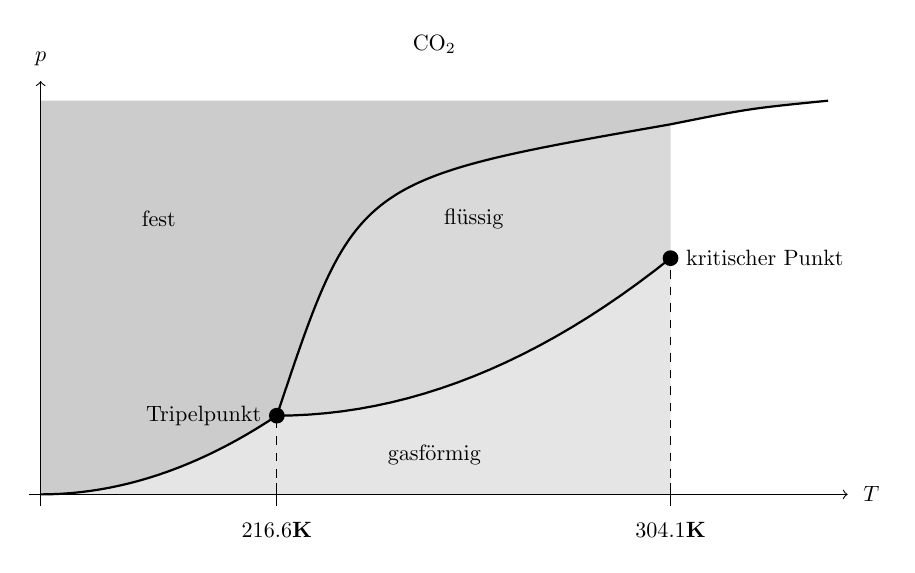
\begin{tikzpicture}[baseline=2.5cm]

  \fill[white!90!black,domain=0:3] (0,0) -- plot (\x,{(\x^2)/9}) -- (3,1) -- (3,0) -- cycle;
  \fill[white!90!black,domain=3:8] (3,0) -- (3,1) -- plot (\x,{2*((\x-3)^2)/25+1}) -- (8,3) -- (8,0) -- cycle;

  \fill[white!80!black,domain=0:3] (0,0) -- plot (\x,{(\x^2)/9}) -- (3,1) .. controls (4,4) .. (8,4.7) .. controls (9,4.9) .. (10,5) -- (0,5) -- cycle;

  \fill[white!85!black,domain=3:8] (3,1) -- plot (\x,{2*((\x-3)^2)/25+1}) -- (8,3) -- (8,4.7) .. controls (4,4) .. (3,1) -- cycle;

  \draw[->] (0,-0.15) to (0,5.25);
  \draw[->] (-0.15,0) to (10.25,0);
  \node[anchor=south] at (0,5.35) {$p$};
  \node[anchor=west] at (10.35,0) {$T$};

  \draw[thick,domain=0:3] plot (\x,{(\x^2)/9});
  \draw[thick,domain=3:8] plot (\x,{2*((\x-3)^2)/25+1});
  \draw[thick] (3,1) .. controls (4,4) .. (8,4.7) .. controls (9,4.9) .. (10,5);

  \draw (3,-0.15) to ++ (0,0.3);
  \draw[dashed] (3,0) to ++ (0,1);
  \node[anchor=north] at (3,-0.25) {$216.6\textbf{K}$};

  \draw (8,-0.15) to ++ (0,0.3);
  \draw[dashed] (8,0) to ++ (0,3);
  \node[anchor=north] at (8,-0.25) {$304.1\textbf{K}$};

  \node[anchor=south] at (5,5.5) {\uline{CO$_2$}};

  \fill[black] (3,1) circle (0.1);
  \fill[black] (8,3) circle (0.1);

  \node at (1.5,3.5) {fest};
  \node at (5.5,3.5) {flüssig};
  \node at (5,0.5) {gasförmig};

  \node[anchor=west] at (8.1,3) {kritischer Punkt};
  \node[anchor=east] at (2.9,1) {Tripelpunkt};

\end{tikzpicture}

\end{figure}
\begin{figure}[H]
  \centering
 \input{5/Graph26.tex}
\end{figure}
\begin{figure}[H]
  \centering
 \tikzset{every node/.style={scale=0.8}}
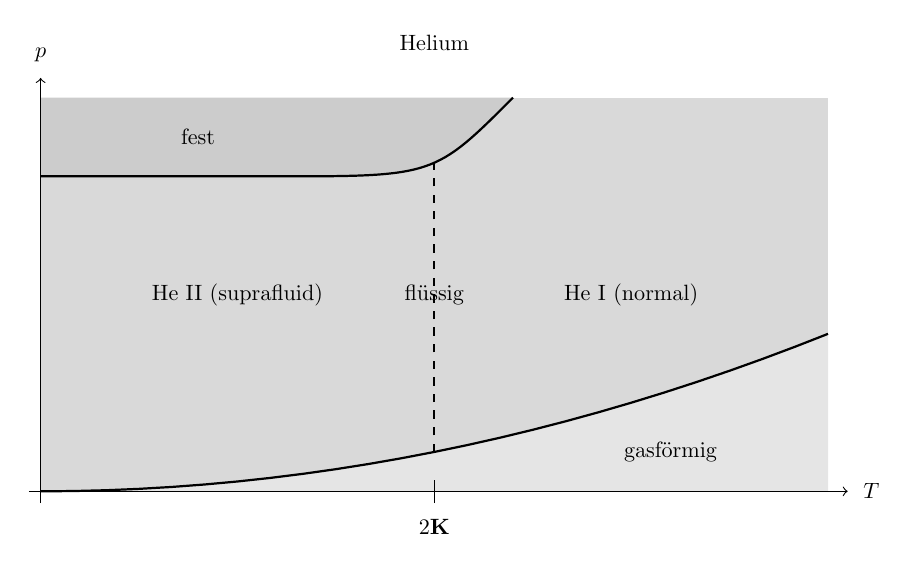
\begin{tikzpicture}[baseline=2.5cm]

  \fill[white!85!black] (0,0) rectangle (10,5);

  \draw[dashed,thick] (5,0.5) to (5,5);

  \fill[white!90!black,domain=0:10] (0,0) -- plot (\x,{(\x^2)/50}) -- (10,2) -- (10,0) -- cycle;

  \fill[white!80!black] (0,4) -- (3,4) .. controls (5,4) .. (6,5) -- (0,5) -- cycle;


  \draw[->] (0,-0.15) to (0,5.25);
  \draw[->] (-0.15,0) to (10.25,0);
  \node[anchor=south] at (0,5.35) {$p$};
  \node[anchor=west] at (10.35,0) {$T$};

  \draw[thick,domain=0:10] plot (\x,{(\x^2)/50});
  \draw[thick] (0,4) -- (3,4) .. controls (5,4) .. (6,5);

  \draw (5,-0.15) to ++ (0,0.3);
  \node[anchor=north] at (5,-0.25) {$2\textbf{K}$};

  \node[anchor=south] at (5,5.5) {\uline{Helium}};

  \node at (2,4.5) {fest};
  \node at (5,2.5) {flüssig};
  \node at (8,0.5) {gasförmig};

  \node at (2.5,2.5) {He II (suprafluid)};
  \node at (7.5,2.5) {He I (normal)};

\end{tikzpicture}

\end{figure}

\begin{itemize}[align=left]
  \item[Typischer Fall:] $p$, $T$, $N$ konstant vorgegeben $\rightarrow$ freie Enthalpie $G$ minimal\\
  Wenn nur $1$ Phase, dann $\mu = \frac{G}{N}$ $\rightarrow$ $\mu$ minimal\\
  Wenn $2$ Phasen, dann $T_1= T_2$, $p_1 = p_2$, $\mu_1 = \mu_2$.
  \item[Im Allgemeinen:] Mehrere Spezies (Molekülsorten), Anzahl $r$; mehrere Phasen, Anzahl $\nu$\\ Jede Spezies $j$ hat ein chemisches Potential $\mu_j = \mu_j^{\norBra{1}} = \dots = \mu_j^{\norBra{\nu}}$ $j = 1, \dots, r$
  \item[$\rightarrow$] $r\cdot\norBra{\nu-1}$ Gleichgewichtsbedingungen
  \item[In jeder Phase] ist $\mu$ eindeutig von den intensiven Variablen festgelegt (Gibbs-Duhem-Relation): $\mu_j^{\norBra{\alpha}} = \mu_j\norBra{T,p,x_1^{\norBra{\alpha}}, \dots, x_{r-1}^{\norBra{\alpha}}}$ mit Anteilen $x_j^{\norBra{\alpha}} = \frac{N_j^{\norBra{\alpha}}}{\sum\limits_{j=1}^r N_j^{\norBra{\alpha}}}$, $\sum\limits_j x_j^{\norBra{\alpha}} = 1$
  \item[$\rightarrow$ Anzahl Variablen:] $2 + \nu\cdot\norBra{r-1}$
  \item[$\rightarrow$ Anzahl Freiheitsgrade (unabhängige intensive Variablen):] $f = 2 + \nu\cdot\norBra{r-1} - r\cdot\norBra{\nu-1}$
  \item[$\rightarrow$] \fbox{$f = 2 + r - \nu$} (\uline{Gibbssche Phasenregel})
  \item[$\rightarrow$] Für ein $1$-komponentiges System ($r=1$) gibt es die Möglichkeiten: \begin{itemize}[align=left]
    \item[$\nu=1$] $f=2$ ($1$ Phase, $p$, $T$ unabhängig variierbar)
    \item[$\nu = 2$] $f=1$ ($2$ Phasen, $p$ von $T$ abhängig)
    \item[$\nu=3$] $f=0$ ($3$ Phasen, $p$ und $T$ fest)
  \end{itemize}
  (maximal 3 Phasen)
\end{itemize}
\uline{Koexistenzkurve beim Gleichgewicht von $2$ Phasen im $1$-komponentigen System}

\begin{figure}[H]
  \centering
  \tikzset{every node/.style={scale=0.8}}
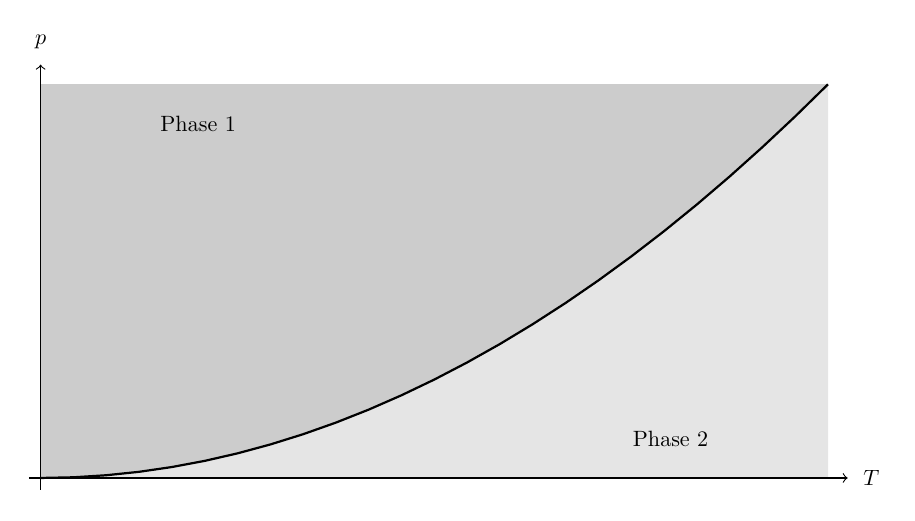
\begin{tikzpicture}[baseline=2.5cm]

  \fill[white!80!black] (0,0) rectangle (10,5);

  \fill[white!90!black,domain=0:10] (0,0) -- plot (\x,{(\x^2)/20}) -- (10,2) -- (10,0) -- cycle;


  \draw[->] (0,-0.15) to (0,5.25);
  \draw[->] (-0.15,0) to (10.25,0);
  \node[anchor=south] at (0,5.35) {$p$};
  \node[anchor=west] at (10.35,0) {$T$};

  \draw[thick,domain=0:10] plot (\x,{(\x^2)/20});

  \node at (2,4.5) {Phase $1$};
  \node at (8,0.5) {Phase $2$};

\end{tikzpicture}

\end{figure}

\begin{itemize}[align=left]
  \item[Gibbs-Duhem:] $\dd{\mu} = - s \dd{T} + v\dd{p}$
  \item[Koexistenzkurve:] $\mu_1 = \mu_2$ für alle $p$, $T$
  \item[$\rightarrow$] $\dd{\mu_1} = \dd{\mu_2}$
  \item[$\rightarrow$] $- s_1 \dd{T} + v_1 \dd{p} = - s_2 \dd{T} + v_2 \dd{p}$
  \item[$\rightarrow$] \fbox{$\ddv{p}{T} = \frac{s_2-s_1}{v_2-v_1}$} \uline{clausius-Clapeyron-Gleichung}
  \item[Entropiedifferenz zwischen Phasen:] $\Delta s = s_2 - s_1$, $l = T \Delta s$
  \item[$l =$] \glqq\uline{latente Wärme}\grqq, \glqq\uline{Verdampfungswärme}\grqq, \glqq\uline{Schmelzwärme}\grqq\ (hier: pro Teilchen)
  \item[$l=$] \uline{Umwandlungsenthalpie} (korrekter Ausdruck, da Vorgang bei konstantem Druck stattfindet)
  \item[$\rightarrow$] $\ddv{p}{T} = \frac{l}{T\Delta v}$
  \item[\uwave{Beispiel}:] Übergang Wasser-Eis $v_\text{Wasser} < v_\text{Eis}$ $\rightarrow$ $\Delta v < 0$ $\rightarrow$ $\ddv{p}{T} < 0$
  \item[Einfachstmögliches Modell für:] Gas $\leftrightarrow$ Flüssigkeit beziehungsweise Gas $\leftrightarrow$  Festkörper: \begin{itemize}[align=left]
    \item[1)] $v_\text{gas} \gg v_\text{fest,flüssig}$ $\rightarrow$ $\Delta v = v_\text{gas}$
    \item[2)] Ideales Gas $\rightarrow$ $v_\text{gas} = \frac{V_\text{gas}}{N_\text{gas}} = \frac{k_B T}{p}$
    \item[1) und 2) $\rightarrow$] $\ddv{p}{T} = l \frac{p}{k_B T^2}$ $\rightarrow$ $p= p_0 e^{-\frac{l}{k_B T}}$
    \item[3)] $l=\text{konstant}$
    \item[Modell] vernachlässigt die Existenz des kritischen Punkts ($l=0$)
  \end{itemize}
\end{itemize}
\begin{figure}[H]
  \centering
  \tikzset{every node/.style={scale=0.8}}
\begin{tikzpicture}[baseline=2.5cm]
  \draw[->] (0,-0.15) to (0,5.25);
  \draw[->] (-0.15,0) to (10.25,0);
  \node[anchor=south] at (0,5.35) {$p$};
  \node[anchor=west] at (10.35,0) {$T$};

  \draw[thick] (0,0) .. controls (5,0) and (6,5) .. (10,5);

\end{tikzpicture}

\end{figure}

\subsection{Dritter Hauptsatz}
(auch: Nernstsches Theorem)
\begin{itemize}[align=left]
  \item[Entropie] kann experimentell durch Messung von Wärmekapazitäten bestimmt werden:\\
  $C_X = T\pdv{S}{T}{X}$ $\rightarrow$ $S\norBra{T} = S\norBra{T_0} + \int\limits_{T_0}^{T} \frac{C_X\norBra{T'}}{T'} \dd{T'}$ ($X = \text{fest}$)
  \item[Empirisch:] Für $T\to 0$ geht $S$ gegen eine endliche Konstante, die nicht von Druck, Phase und so weiter abhängt. $\rightarrow$ Setze Konstante $=0$.
\end{itemize}
$\rightarrow$ \uline{Dritter Hauptsatz}\\
\fbox{\parbox{0.98\textwidth}{Am absoluten Nullpunkt $T=0$ ist die Entropie $S=0$. Das heißt für isotherme Prozesse bei $T\to 0$ gilt $\Delta S \to 0$.}}\\
Damit $S\norBra{T=0}$ einen endlichen Wert hat, muss gelten $\verBra{\int\limits_0^T \frac{C_X\norBra{T'}}{T'}\dd{T'}} < \infty$ und daher $C_X\norBra{T} \stackrel[T\to 0]{ }{\rightarrow} 0$. (Alle Wärmekapazitäten verschwinden bei $T=0$.)

\begin{itemize}[align=left]
  \item[Ausdehnungskoeffizient:] $\alpha = \frac{1}{V} \pdv{V}{T}{p} = - \frac{1}{V}\pdv{S}{p}{T} \to 0$ für $T\to 0$\\
  $\frac{\alpha}{\kappa_T} = \frac{\pdv{S}{p}{T}}{\pdv{V}{p}{T}} = \pdv{S}{V}{T} \to 0$ für $T\to 0$
  \item[Wie] kann man sich dem absoluten Nullpunkt annähern?
  \item[Adiabatische Expansion:] $\dd{T} = \pdv{T}{p}{S} \dd{p}$ (genauer: isentropisch)
  \item[$\pdv{T}{p}{S}$] $= \ppv{\norBra{T,S}}{\norBra{p,S}} = \ppv{\norBra{T,S}}{\norBra{p,T}}\ppv{\norBra{p,T}}{\norBra{p,S}} = - \frac{\pdv{S}{p}{T}}{\pdv{S}{T}{p}} = \frac{V\alpha}{\frac{C_p}{T}}$
  \item[$\rightarrow$] $\dd{T} = \frac{V\alpha T}{C_p}\dd{p}$
  \item[$\frac{V\alpha T}{C_p}$] $\stackrel[T\to 0]{}{\rightarrow} 0$ woraus folgt $\frac{V\alpha}{C_p} \stackrel[T\to 0]{}{\rightarrow} \text{konstant} \neq 0$, denn
  \begin{itemize}[align=left]
    \item[$V\alpha$] und $C_p$ gehen \glqq gleich schnell\grqq\ gegen Null: $S\stackrel[T\to 0]{}{\sim} T^{\times}$
    \item[$\rightarrow$] $V\alpha = -\pdv{S}{p}{T} \sim T^{\times}$, $C_p = T \pdv{S}{T}{p} \sim T^{\times}$
  \end{itemize}
  \item[$\rightarrow$] Nullpunkt kann nicht durch adiabatische Expansion erreicht werden.\\
  Es muss außerdem die Entropie verringert werden durch Wärmeabfuhr. Dazu muss ein ebenso kaltes Wärmebad vorhanden sein.
  \item[$\rightarrow$] Man kann den Nullpunkt nicht (in endlich vielen Teilschritten) erreichen. (Alternative Formulierung des 3. Hauptsatzes.)
\end{itemize}

\begin{figure}[H]
  \centering
  \tikzset{every node/.style={scale=0.8}}
\begin{tikzpicture}[baseline=2.5cm]
  \draw[->] (0,-0.15) to (0,5.25);
  \draw[->] (-0.15,0) to (10.25,0);
  \node[anchor=south] at (0,5.35) {$T$};
  \node[anchor=west] at (10.35,0) {$S$};

  \draw[thick] (3,0) to (4,5);
  \draw[thick] (3,0) to (6,3);

  \draw[thick,->] (8,5) to (4,5);
  \draw[thick,->] (4,5) to (4,1);
  \draw[thick,->] (4,1) to (3.2,1);
  \draw[thick,->] (3.2,1) to (3.2,0.2);
  \node[anchor=south] at (6,5.1) {Wärmeentnahme};
  \node[anchor=west] at (4.1,3.5) {adiabatische Abkühlung};

\end{tikzpicture}

\end{figure}

\uline{Statistische Erklärung}:\\
Bei $T=0$ ist nur der niedrigste Quantenzustand besetzt ($P_j \sim e^{-\frac{E_j}{k_B T}}$). Wenn Grundzustand nicht-entartet, dann $S\norBra{T=0} = 0$, wenn $g_0$ entartete Grundzustände, dann $S\norBra{T=0} = k_B \ln g_0$.
\begin{itemize}[align=left]
  \item[Übliche Annahme:] Tatsächilcher Grundzustand nicht-entartet, wird aber in der Praxis nicht erreicht $\rightarrow$ Restentropie.
  \item[Klassische Ergebnisse:] im Widerspruch zum 3. Hauptsatz
\end{itemize}

\subsection{Thermodynamischer Limes, Zusammenfassung}
\begin{itemize}[align=left]
  \item[* \uline{Thermodynamischer Limes}:] Teilchenzahl $N\to\infty$, so dass extensove Variablen $\to\infty$ und intensive Variablen $\to\text{konstant}$.\\
  In diesem Fall stimmen die Vorhersagen verschiedener Ensembles ($=$ Gesamtheiten) überein.
  \item[*] Thermodynamik kann unabhängig von statistischer Physik formuliert werden (Hauptsätze), aber stimmt mit ihr überein. Theorie der \uline{Gleichgewichtszustände}.
  \item[*] Zentrale Größe: \uline{Entropie} $\rightarrow$ Definitione für $T$, $p$, $\mu$.
  \item[*] 2. Hauptsatz $\rightarrow$ \uline{Stabilitätsbedingungen}
  \item[\uwave{Nachtrag}:] Seit 2019 sind Boltzmannkonstante $k_B$, Avogadrozahl $N_A$ und universelle Gaskonstante $R = k_B \cdot N_A$ exakt festgelegt: $k_B = 1.380649\cdot 10^{-23}\frac{\textbf{J}}{\textbf{K}}$, $N_A = 6.02214076\cdot 10^{23} \textbf{mol}^{-1}$
\end{itemize}
